\documentclass[11pt,letterpaper]{article}
%\usepackage{fullpage}
\usepackage[top=2cm, bottom=4.5cm, left=2.5cm, right=2.5cm]{geometry}
\usepackage{amsmath,amsthm,amsfonts,amssymb,amscd}
%\usepackage{lastpage}
\usepackage{enumerate}
\usepackage{subcaption}
%\usepackage{fancyhdr}
%\usepackage{mathrsfs}
\usepackage{xcolor}
\usepackage{graphicx}
\usepackage{listings}
\usepackage{hyperref}
\usepackage{listings}
\usepackage{comment}
\lstset{
   breaklines=true,
   basicstyle=\ttfamily}
\usepackage{spverbatim}
\usepackage{pdfpages}
\usepackage{tikz}
\hypersetup{%
  colorlinks=true,
  linkcolor=blue,
  linkbordercolor={0 0 1}
} 
\usepackage{enumitem}

\lstdefinestyle{Python}{
    language        = Python,
    frame           = lines, 
    basicstyle      = \footnotesize,
    keywordstyle    = \color{blue},
    stringstyle     = \color{green},
    commentstyle    = \color{red}\ttfamily
}

\setlength{\parindent}{0.0in}
\setlength{\parskip}{0.05in}

% Edit these as appropriate
\newcommand\course{ISyE 719}
\newcommand\hwnumber{3}                  % <-- homework number
\newcommand\NetIDa{}           % <-- NetID of person #1
\newcommand\NetIDb{}           % <-- NetID of person #2 (Comment this line out for problem sets)

%\pagestyle{fancyplain}
%\headheight 35pt
%\lhead{\NetIDa}
%\lhead{\NetIDa\\\NetIDb}                 % <-- Comment this line out for problem sets (make sure you are person #1)
%\chead{\textbf{\Large \course \text{ }Project Submission}}
%\rhead{\course \\ \today}
%\lfoot{}
%\cfoot{}
%\rfoot{\small\thepage}
%\headsep 1.5em


\begin{document}

\begin{comment}
% Deadline 1: March 29, a brief write up\\
% Deadline 2: April 4/5- A slightly concrete proposal\\
% Deadline 3: April 6-Write up each other's parts. \\
% Deadline 4: April-6 Mail proposal by midnight . 


% Meeting Scheduled on April 6-5pm\\
% Short meeting on April 6 - 7pm. (Discuss proposal and next meeting) 

% \href{http://www.optimization-online.org/DB_FILE/2015/08/5064.pdf}{sddp paper}\\
% \href{https://www.ima.umn.edu/materials/2015-2016/ND8.1-12.16/25386/mssp.pdf}{shabbir}\\
% \href{https://www.ima.umn.edu/2015-2016/ND8.1-12.16/25386}{Shabbir's Video}\\
% \href{https://www.reuters.com/article/us-health-coronavirus-usa-ventilators/outbid-and-left-hanging-u-s-states-scramble-for-ventilators-idUSKCN21S20D}{Unreliable data}
% \href{https://covid19.healthdata.org/united-states-of-america}{ihme data}
\end{comment}

\title{Stochastic Programming Approach to Temporal Resource Allocation for COVID-19 Pandemic.}
\date{}
\author{Akhilesh Soni, Bhumesh Kumar}
\maketitle
\section{Introduction}
In this work we aim to study, implement and extend stochastic programming models and algorithms for temporal resource sharing during pandemic across a finite time horizon.  Efficient resource allocation is a fundamental problem in supply chain, manufacturing, telecommunication, military, online resource sharing, and other areas (See \href{https://apps.dtic.mil/dtic/tr/fulltext/u2/a423115.pdf}{Temporal resource Allocation}, \href{https://arxiv.org/pdf/1610.02143.pdf}{Online Resource Allocation}). The problem of sharing super-critical and scarce resources (e.g. Ventilators, testing kits) is of particular interest towards crisis management in health care for patient care as well as triage.   
%\href{https://people.orie.cornell.edu/huseyin/publications/informs_tutorial_formatted.pdf}{Solving SP using Dynamic Prog. for Resource Allocation}. 

Our project is motivated by the recent global pandemic, COVID-19; challenges USA and other economies are encountering in medicare and public health through the pandemic. For patients with underlying illnesses or of elder ages, the effects of COVID-19 on respiratory systems can be fatal (See \href{http://www.optimization-online.org/DB_FILE/2020/04/7719.pdf}{Mehrotra et al.}). The supply of Oxygen for the body may not be enough for the time patient is undergoing recovery and thus ventilators are a critical resource for ensuring patient survival. 

The speed of the pandemic, ease of spread and manufacturing limitations both cost and speed make ventilators a scarce resource. This presses an impending need for efficient sharing of ventilators and other resources. Over the course of pandemic, such resource pooling can have a significant effect on reducing the number of death toll as well as the nation's economy.  

Resource allocation has been classically studied in multiple fields, spanning
\href{https://eprints.illc.uva.nl/168/}{economics},
\href{https://dl.acm.org/doi/book/10.5555/1457343}{wireless networks},
\href{https://link.springer.com/chapter/10.1007/978-1-349-24002-9_5}{game theory},
\href{https://ideas.repec.org/a/eee/jrpoli/v22y1996i3p218-220.html}{finance} etc. 
and focus on one shot allocation in deterministic, stochastic and adversarial settings. 
The outbreak of pandemic typically follows a bell curve with each state/region of the country hitting the peak at different points of time. 
This lends the problem a time dependent structure where in each time horizon, resource can be re-located and/or shared based on the projected need. 

Optimization techniques have been explored for 
\href{https://www.ncbi.nlm.nih.gov/pubmed/18700149}{vaccinations},
\href{http://www2.pitt.edu/~schaefer/papers/FluShotDesign.pdf}{influenza treatments} etc. Stochastic programming and \href{https://www.sciencedirect.com/science/article/abs/pii/0025556479900828}{optimal control} are the popular paradigms to model and target these issues. \href{https://www.sciencedirect.com/science/article/pii/S1755436514000280}{Challenges} in modelling and applicability of assumptions have also been studied. 

In a \href{https://pubsonline.informs.org/doi/pdf/10.1287/trsc.2017.0777}{recent paper} by Mehrotra et. al., authors solve a ventilator re-location problem using a multi period planning model. They model uncertainty in the demands which are observable only after the relocation decision has been made. Decision making lies in determining the number of ventilators that are moved from location A to location B in each time period and authors solve an extensive formulation model considering 4 possible demand scenarios. The decision maker makes a decisions for the entire planning horizon using the information that is available at the beginning of planning. 

\subsection*{Problem Description}
During the course of a pandemic, different regions of the country hit peak demand of necessary healthcare equipments like ventilators, hospital bed etc. Our focus in this work is on the ventilators and we restrict our geographical region to United States of America. We show the predicted mean demand curve for each state in Figure \ref{fig:meanDemand}. Note that we pulled the data from Institute for Health and Metrics \href{http://www.healthdata.org/covid/data-downloads}{IHME} website.Note that this data is for the number of additional ventilators required by each state i.e the unmet demand each state is expected to have.
As each states hits it's peak demand at a different point of time, ventilators can be shared among various states if planning is done efficiently. It is difficult to predict the demand of ventilators in each state with high accuracy. Hence, a need arises for a model which can provide efficient ways for resource ventilators amidst this uncertain demand. Our work is a major extension of   
 \href{http://www.optimization-online.org/DB_FILE/2020/04/7719.pdf}{Mehrotra et al.}. We propose a novel multi-stage stochastic program formulation for the ventilator relocation problem. We then use stochastic dual dynamic programming (SDDP) algorithm to solve the model efficiently. Note that as number of scenarios increase, solving extensive form becomes impossible.
 \begin{figure}[h!]
    \centering
    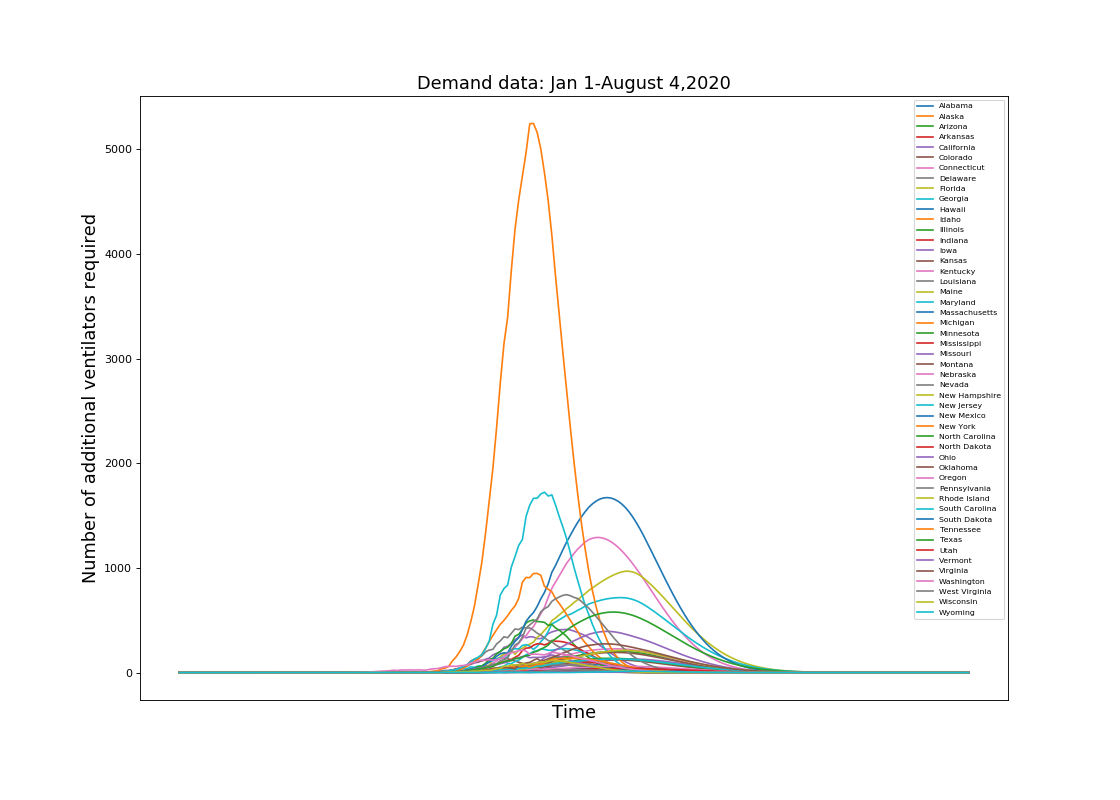
\includegraphics[scale=0.5]{demand-data.png}
    \caption{Mean demand curves from Jan 1-Aug 4, 2020 (Source:IHME)}
    \label{fig:meanDemand}
\end{figure}
 \section{Mathematical Model}
 In this section we provide model
 \subsection{Modeling Assumptions}
 \begin{itemize}
     \item As number of ventilators is a large qualtity, we can round it of to a nearest integer. Thus we assume the number of ventilators to be continuous instead of discrete. 
     \item We assume lead time to be zero. We consider our period length to be 1 week. 
     \item We treat penalty of unmet demand to be a constant i.e. it doesn't vary from state to state
     \item We assume that the demand in first period is known with certainty in each state
 \end{itemize}
\subsection{Notation}
\paragraph{Sets and Parameters}
\begin{itemize}
    \item $S\rightarrow$ Set of states/ regions
    \item $T \rightarrow$ Set of periods
    \item $K \rightarrow$ Set of scenarios
   \item $i_s\rightarrow$ Starting inventory of each state 
   \item $p\rightarrow$ Penalty for each unit of unmet demand, (purchasing a new ventilator)
   \item $c_{s_1,s_2}\rightarrow$ Cost of transporting a ventilator from state $s_1$ to state $s_2$
   \item $\mu^t_s\rightarrow$ Mean demand in period t in state $s\in S$ is known
   \item $\omega \rightarrow$ Timeseries parameter
  \item $f^1_s\rightarrow$ Demand multiplicative factor in period 1 in state $s$

\end{itemize}

\paragraph{Stochastic Data}
\begin{itemize}
    \item $\xi^t_s \rightarrow$Random Variable, $LogN(1,0.15)$.This is used to induce uncertainty in demand and create different scenario demand.
   \item $d^t_s\rightarrow$ Demand in period $t\ge 2$ in state $s$
\end{itemize}

\paragraph{Decision variables}
\begin{itemize}
    \item $x^t_{s_1,s_2}\rightarrow$Number of ventilators moved from states $s_1$ to state $s_2$ in period t-\textcolor{blue}{State Variable}
    \item $u^t_s\rightarrow$Ventilators held by state s in period t-\textcolor{blue}{State Variable}
    \item $f^t_s\rightarrow$Demand multiplication factor in stage t in state s-\textcolor{blue}{State Variable}
    \item $y^t_s\rightarrow$Ventilators available in state s in period t which are not in use-\textcolor{blue}{Recourse Variable}
    \item $z^t_s\rightarrow$Unmet demand in state s in period t-\textcolor{blue}{Recourse Variable}
\end{itemize}

\subsection{Demand Model}
We know that demand follows the shape of bell curve as clear from Figure \ref{fig:meanDemand}. Moreover, IHME also provides possible variation in demand data i.e. min and max. We show in Figure \ref{fig:demandVariation} the minimum, maximum, and mean demand predictions by IHME for the state of New York, New Jersey, Massachusetts, and Connecticut.
\begin{figure}[h!]
  \centering
  \begin{subfigure}[b]{0.45\linewidth}
    \includegraphics[width=\linewidth]{New York-dev.png}
    \caption{New York}
  \end{subfigure}
  \begin{subfigure}[b]{0.45\linewidth}
    \includegraphics[width=\linewidth]{New Jersey-dev.png}
    \caption{New jersey}
  \end{subfigure}
  \begin{subfigure}[b]{0.45\linewidth}
    \includegraphics[width=\linewidth]{Massachusetts-dev.png}
    \caption{Massachusetts}
  \end{subfigure}
  \begin{subfigure}[b]{0.45\linewidth}
    \includegraphics[width=\linewidth]{Connecticut-dev.png}
    \caption{Connecticut}
  \end{subfigure}
  
  \caption{Demand Variation with time}
  \label{fig:demandVariation}
\end{figure}
\newline 
To capture this behaviour, we use the following multiplicative auto regressive time series model. 
\begin{align}
d^t_{s}&=\mu^{t}_{s}*f^t_s \qquad \forall t\ge 2,s\in S\\
f^t_s&=\omega f^{t-1}_s+(1-\omega)\xi^t_s \qquad \forall t\ge 2, s\in S\\
&\xi^t_s\in LogN(1,0.15)\\
&\omega\in (0,1) \text{is a fixed parameter}
\end{align}
Note that $\omega$ here is regression parameter and $\xi^t_s$ is the noise
\subsection{Extensive Formulation}
We provide an extensive model formulation in this section. Consider that we have a possible list of scenarios in set $K$ i.e. set $K$ comprised of various demand scenarios for each state across all the periods. Let demand scenario $k$ occurs with a probability of $p^k$
\begin{align*}
    \min & \sum_{t\in T}\sum_{s\in S}\big[\sum_{s_2 \in s, s_2\neq s} c_{s,s_2}x^t_{s,s_2}+\sum_{k\in K} p^kpz^t_{sk}\big]\\
    \text{s.t. } & u_s^t=u_s^{t-1}+\sum_{s_2\in S,s_2\neq s}x^t_{s_2,s}-\sum_{s_2\in S, s_2\neq s}x^t_{s,s_2} \qquad \forall t\ge 2, \forall s \in S\\
    & u_s^1=i_s \qquad \forall s\in S\\
    %& z^{t}_s+u^t_s \ge d^{t}_s \qquad \forall t\in T,s \in S\\
    & z^t_s+u^t_s=f^t_s\mu^t_s+y^t_{sk} \qquad \forall t \in T,s \in S, k\in K\\
    &f^t_s=\omegaf^{t-1}_s+(1-\omega)\xi^t_{s,k} \qquad \forall s\in S, t\ge 2,k\in K \\
    &f^1_s=d^1_s \qquad \forall s\in S\\
    & \sum_{s_2\in S}x^t_{s,s_2}\le y^t_{sk} \qquad \forall s \in S, t\in T, k\in K\\
    & x^t_{s_1,s_2}, u^t_s,y^t_{sk},z^t_{sk} \geq 0 \qquad s\in S, t\in T,k \in K
\end{align*}
\subsection{Stochastic Dual Dynamic Programming}
As the number of scenarios increase, the extensive form model becomes intractable. Hence, in this section we propose a SDDP algorithm for this model.
\subsection*{Forward Pass}
In each iteration of forward pass we generate a sample path say $P_i$ which provides a random noise realization ($\xi^t_{si}$) for each states $s$ in each period $t$. We then solve the following deterministic period in each stage while using the solution from previous stage as an input.
Thus, we solve the forward pass problem in iteration $i$
\begin{align}
    (x^t,u^t,y^t,z^t) \in \argmin_{x,u,y,z,\theta} & \sum_{s\in S}\big[\sum_{s_2 \in s, s_2\neq s} c_{s,s_2}x_{s,s_2}+pz_{s}\big]+\theta\\
    \text{s.t. } & u_s=\textcolor{red}{{\hat{u}}_s^{t-1}}+\sum_{s_2\in S,s_2\neq s}x_{s_2,s}-\sum_{s_2\in S, s_2\neq s}x_{s,s_2} \qquad \forall \forall s \in S\\
    %& u_s^1=i_s \qquad \forall s\in S\\
    %& z^{t}_s+u^t_s \ge d^{t}_s \qquad \forall t\in T,s \in S\\
    & z_s+u_s=\mu^{t}_{s}*f_s+y_s \qquad \forall s \in S\\
    &f_s=\omega \textcolor{red}{\hat{f}^{t-1}_s}+(1-\omega)\xi^t_{s,\textcolor{red}{P_i}} \qquad \forall t\ge 2\\
    & \sum_{s_2\in S}x_{s,s_2}\le y_{s} \qquad \forall s \in S\\
    & x_{s_1,s_2}, u_s,y_s,z_s\ge 0 \\
    & \textcolor{blue}{\theta\ge \frac1N \Big[\sum_{j'}\alpha^l_{j',t+1}+\sum_{j'}\sum_s\rho^l_{s,j',t+1}{u}_s +\omega\sum_{j'}\sum_s\gamma^l_{s,j',t+1}{f}_s \Big]} \quad \forall l=1,\dots,i-1 \tag{Benders Cut-fp}
\end{align}
Note that ${\hat{u}}_s^{t-1}$ and ${\hat{f}}_s^{t-1}$ are solutions from previous stage. 

\subsection*{Backward Pass Pass}
In backward pass, we start from last stage and work our way towards first stage. All scenario problems are solved each stage in backward pass i.e. we solve the following problem for each scenario ($j$).
In stage $t+1$, we use stage solution from past stage($t$) and expected go to function approximation (approximation, $\theta$) from future($t+2$)
\begin{align}
    \Q^{i+1}_{j,t+1}=\min_{x,u,y,z,\theta} & \sum_{s\in S}\big[\sum_{s_2 \in s, s_2\neq s} c_{s,s_2}x_{s,s_2}+pz_{s}\big]+\theta\\
    \text{s.t. } & u_s-\sum_{s_2\in S,s_2\neq s}x_{s_2,s}+\sum_{s_2\in S, s_2\neq s}x_{s,s_2}=\textcolor{red}{{\hat{u}}_s^{t}} \qquad \forall s \in S \tag{$\rho^i_{s,j,t+1}$}\\
    %& u_s^1=i_s \qquad \forall s\in S\\
    %& z^{t}_s+u^t_s \ge d^{t}_s \qquad \forall t\in T,s \in S\\
    & z_s+u_s-y_s-\mu^{t+1}_s*f_s=0 \qquad \forall s \in S \\
    &f_s=\omega \textcolor{red}{\hat{f}^{t}_s}+(1-\omega)\xi^{t+1}_{s,\textcolor{red}{j}} \qquad \forall s\in S \tag{$\gamma^i_{s,j,t+1}$}\\
    & \sum_{s_2\in S}x_{s,s_2}- y_{s}\le 0 \qquad \forall s \in S \\
    & x_{s_1,s_2}, u_s,y_s,z_s\ge 0\\
    & \textcolor{blue}{\theta\ge \frac1N \Big[\sum_{j'}\alpha^l_{j',t+2}+\sum_{j'}\sum_s\rho^l_{s,j',t+2}{u}_s +\omega\sum_{j'}\sum_s\gamma^l_{s,j',t+2}{f}_s\Big]} \quad \forall l=1,\dots,i \tag{Benders Cut-bp}
\end{align}
We associate the dual variables $\rho^i_{s,j,t+1}$ and $\gamma^i_{s,j,t+1}$ with two sets of constraints as shown in abose equations.
We then calculate $\alpha^i_{j,t+1}$ as following which is used to generate benders cut.
\begin{align}
    &\alpha^i_{j,t+1}=\Q^{i+1}_{j,t+1}-\sum_s\rho^i_{s,j,t+1}{\hat{u}}^t_s-\omega\sum_s\gamma^i_{s,j,t+1}{\hat{f}}^t_s
\end{align}
Add cut to all nodes in t:
\begin{align}
    \theta \ge \frac1N \Big[\sum_{j'}\alpha^i_{j',t+1}+\sum_{j'}\sum_s\rho^i_{s,j',t+1}{u}^t_s+\omega\sum_{j'}\sum_s\gamma^i_{s,j',t+1}{f}^t_s \Big]
\end{align}

\section{Computational Results}
In this section we share computational results.
\subsection{Data}
We use data from \href{https://pubsonline.informs.org/doi/pdf/10.1287/trsc.2017.0777}{Mehrotra et al.}. Our data comprises of current inventory in state and federal reserves, willingness of each state to share it's resources with another state, expected arrival of new ventilators being manufactured, and varying demand scenarios for each state/regions

\begin{comment}

\section{Not in report}
Anything after this point is old material. Copy paste from below and structure the report properly.
 \section*{Meeting with Jim on April 10}
factor in the travel time and when will be they available.Keeping track of how long have been they in use. Try SDDP maybe if demands are iid (Might be challenging). Clustering by regions maybe to reduce the size of the problem. For SDDP, d(t)=d(history)+some error function-auto regressive model. Error has some dependency. Mail challenge is figuring out how to fit the demand variable in SDDP framework. Scenario tree model not good enough because of too many states.
Markov chain might be a good approximation for keeping track of number of infections. Growth rate can depend on time (in a deterministic manner). Julia SDDP has some implemented algorithms. Comparison of different approaches, need a simulation to compare (beyomd the scope of the project). Implementing one algorithm might be enough. Goal should be to minimize the unmet demand (expected value or some risk measures)


%%%%%%%%%%%%%%%%%%%%%%%%%%%%%%%%%%%%%%%%%%%%%%%%%%%%%%%%%%%%%%%%%%%%%%%%%%%%%%%%%%%%%%%%%%%%%%%%%%%%%%%%%%%%%%%%%%%%%%%%

\subsection*{Proposed Theme}
Stochastic Programming Approach to Temporal Resource Allocation for COVID-19 Pandemic.

\subsection*{Abstract}
This project aims to study, implement and extend stochastic programming models and algorithms for temporal resource sharing during pandemic across a finite time horizon.  

\subsection*{Introduction and Motivation}
Efficient resource allocation is a fundamental problem in supply chain, manufacturing, telecommunication, military, online resource sharing, and other areas (See \href{https://apps.dtic.mil/dtic/tr/fulltext/u2/a423115.pdf}{Temporal resource Allocation}, \href{https://arxiv.org/pdf/1610.02143.pdf}{Online Resource Allocation}). The problem of sharing super-critical and scarce resources (e.g. Ventilators, testing kits) is of particular interest towards crisis management in health care for patient care as well as triage.   
%\href{https://people.orie.cornell.edu/huseyin/publications/informs_tutorial_formatted.pdf}{Solving SP using Dynamic Prog. for Resource Allocation}. 

Our project is motivated by the recent global pandemic, COVID-19; challenges USA and other economies are encountering in medicare and public health through the pandemic. For patients with underlying illnesses or of elder ages, the effects of COVID-19 on respiratory systems can be fatal (See \href{http://www.optimization-online.org/DB_FILE/2020/04/7719.pdf}{Mehrotra et al.}). The supply of Oxygen for the body may not be enough for the time patient is undergoing recovery and thus ventilators are a critical resource for ensuring patient survival. 

The speed of the pandemic, ease of spread and manufacturing limitations both cost and speed make ventilators a scarce resource. This presses an impending need for efficient sharing of ventilators and other resources. Over the course of pandemic, such resource pooling can have a significant effect on reducing the number of death toll as well as the nation's economy.  

\subsection*{Prior Work}
Resource allocation has been classically studied in multiple fields, spanning
\href{https://eprints.illc.uva.nl/168/}{economics},
\href{https://dl.acm.org/doi/book/10.5555/1457343}{wireless networks},
\href{https://link.springer.com/chapter/10.1007/978-1-349-24002-9_5}{game theory},
\href{https://ideas.repec.org/a/eee/jrpoli/v22y1996i3p218-220.html}{finance} etc. 
and focus on one shot allocation in deterministic, stochastic and adversarial settings. 
The outbreak of pandemic typically follows a bell curve with each state/region of the country hitting the peak at different points of time. 
This lends the problem a time dependent structure where in each time horizon, resource can be re-located and/or shared based on the projected need. 

Optimization techniques have been explored for 
\href{https://www.ncbi.nlm.nih.gov/pubmed/18700149}{vaccinations},
\href{http://www2.pitt.edu/~schaefer/papers/FluShotDesign.pdf}{influenza treatments} etc. Stochastic programming and \href{https://www.sciencedirect.com/science/article/abs/pii/0025556479900828}{optimal control} are the popular paradigms to model and target these issues. \href{https://www.sciencedirect.com/science/article/pii/S1755436514000280}{Challenges} in modelling and applicability of assumptions have also been studied. 

In a \href{https://pubsonline.informs.org/doi/pdf/10.1287/trsc.2017.0777}{recent paper}, authors solve a ventilator re-location problem using a multi period planning model. They model uncertainty in the demands which are observable only after the relocation decision has been made. Decision making lies in determining the number of ventilators that are moved from location A to location B in each time period and authors solve an extensive formulation model considering 4 possible demand scenarios. The decision maker makes a decisions for the entire planning horizon using the information that is available at the beginning of planning. 




\subsection*{Proposed Goals and Deliverables for the Project}
%Building on Section \ref{sec: Resource Allocation}.\\
We plan to extend the work of \href{http://www.optimization-online.org/DB_FILE/2020/04/7719.pdf}{Mehrotra et al.} and \textbf{propose a multi-stage stochastic program} while assuming number of resources to be continuous instead of discrete. 
There are known algorithms for solving multi-stage stochastic programs like Rolling Horizon heuristic (2 stage+rolling horizon), Scenario Decomposition (PH), and stagewise Decomposition (SDDP and Nested Benders). We plan to explore and \textbf{study these methods}, and then \textbf{implement a decomposition technique and compare it with the rolling horizon heuristic} (solving multiple 2 stage SP in rolling horizon). If time permits, we will also study the same problem with integral restrictions on the quantity of resources (which is more practical). %However, SMIP in multistage setting are known to be computationally challenging and might be ambitious in the given time frame. 

The second part of the project is to incorporate a risk sensitive perspective and \textbf{propose} a more pragmatic \textbf{chance constrained formulation for the multi-period planning problem}. We follow this with a \textbf{literature survey of methods} proposed for solving such formulations. From our side, we plan to \textbf{propose a version big-M relaxation} with multi-period constraints.    

We plan to use data from \href{https://pubsonline.informs.org/doi/pdf/10.1287/trsc.2017.0777}{Mehrotra et al.}. Our data will comprise of current inventory in state and federal reserves, willingness of each state to share it's resources with another state, expected arrival of new ventilators being manufactured, and varying demand scenarios for each state/region.
 \section*{Meeting with Jim on April 10}
factor in the travel time and when will be they available.Keeping track of how long have been they in use. Try SDDP maybe if demands are iid (Might be challenging). Clustering by regions maybe to reduce the size of the problem. For SDDP, d(t)=d(history)+some error function-auto regressive model. Error has some dependency. Mail challenge is figuring out how to fit the demand variable in SDDP framework. Scenario tree model not good enough because of too many states.
Markov chain might be a good approximation for keeping track of number of infections. Growth rate can depend on time (in a deterministic manner). Julia SDDP has some implemented algorithms. Comparison of different approaches, need a simulation to compare (beyomd the scope of the project). Implementing one algorithm might be enough. Goal should be to minimize the unmet demand (expected value or some risk measures)
\section*{Meeting April 17}
Starting inventory evenly distributed. 
Bhumesh is gonna look after 2-stage, rolling horizon, and risk measures. Pulling up distance between different states.
Akhilesh is going to work on sddp. Do block-wise increasing demand distribution.
Variable for Purchasing ventilators can be a future direction.
Figure out geographical aggregation-there might be too many nodes if we do on a state level
\section*{Meeting April 27}
The demand should be modeled as following:
\begin{align}
d^t_{s}&=\mu^{t}_{s}*f^t_s\\
f^t_s&=\omega f^{t-1}_s+(1-\omega)\xi^t_s \qquad \forall t\ge 2\\
&f^1_s\in N(1,0.15)\\
&\xi^t_s\in LogN(1,0.15)\\
&\omega\in (0,1) \text{is a fixed parameter like 0.8}
\end{align}

\section{Old Model}
\paragraph{Assumptions}
\begin{itemize}
    \item Unmet demand is equivalent to purchasing a new ventilator. We assume that we can meet any unmet demand by purchasing new ventilators.
    \item Demand in period t ($d_t$) depends only on demand in period $t-1$.
    \item We assume that lead time for transportation is 0
\end{itemize}
\paragraph{Sets}
\begin{itemize}
    \item $S\rightarrow$ Set of states/ regions
    \item $T \rightarrow$ Set of periods
\end{itemize}
\paragraph{Parameters}
\begin{itemize}
   \item $i_s\rightarrow$ Starting inventory of each state 
   \item $p\rightarrow$ Penalty for each unit of unmet demand, (purchasing a new ventilator)
   \item $c_{s_1,s_2}\rightarrow$ Cost of transporting a ventilator from state $s_1$ to state $s_2$
   \item $d^1_s\rightarrow$ Demand in period 1 in state $s\in S$ is known
\end{itemize}
\paragraph{Stochastic data}
\begin{itemize}
    \item $\xi_t\rightarrow$Uncertainty to be revealed in period t 
    \item $d^t_s\rightarrow$Demand in state s in period t,$d^t_s=d^{t-1}_{s}+f(\xi^t)$

\end{itemize}
\paragraph{Decision variables}
\begin{itemize}
    \item $x^t_{s_1,s_2}\rightarrow$Number of ventilators moved from states $s_1$ to state $s_2$ in period t-\textcolor{blue}{State Variable}
    \item $u^t_s\rightarrow$Ventilators held by state s in period t-\textcolor{blue}{State Variable}
    \item $y^t_s\rightarrow$Ventilators available in state s in period t which are not in use-\textcolor{blue}{Recourse Variable}
    \item $z^t_s\rightarrow$Unmet demand in state s in period t-\textcolor{blue}{Recourse Variable}
\end{itemize}
\subsection{Scenario Formulation-Extensive Formulation}
\begin{align}
    \min & \sum_{t\in T}\sum_{s\in S}\big[\sum_{s_2 \in s, s_2\neq s} c_{s,s_2}x^t_{s,s_2}+pz^t_{s}\big]\\
    \text{s.t. } & u_s^t=u_s^{t-1}+\sum_{s_2\in S,s_2\neq s}x^t_{s_2,s}-\sum_{s_2\in S, s_2\neq s}x^t_{s,s_2} \qquad \forall t\ge 2, \forall s \in S\\
    & u_s^1=i_s \qquad \forall s\in S\\
    %& z^{t}_s+u^t_s \ge d^{t}_s \qquad \forall t\in T,s \in S\\
    & z^t_s+u^t_s=d^t_s+y^t_s \qquad \forall t \in T,s \in S\\
    & \sum_{s_2\in S}x^t_{s,s_2}\le y^t_s \qquad \forall s \in S\\
    & x^t_{s_1,s_2}, u^t_s,y^t_s,z^t_s \geq 0
\end{align}
Add scenario index(k) to decision variables. Each realization (scenario) has a corresponding probability. Each scenario consists of demand information over all the periods. This is deterministic equivalent. 

We add non anticpativity constraints on state variables such that current decision don't depend on information from future:
\[ u^t_{s,k}=u^t_{s,k'}, y^t_{s,k}=y^t_{s,k'}\]
where k and k' are scenarios which are not distinguishable upto point t. (stages are different from time periods). Might have to build a scenario tree to get better intuition.


\subsection{2 stage Approximation}
First stage=First period. We can then separate by scenario sub  problems. i.e. we solve for t=1, obtain a solution for first stage, move to t=2 with decision for t=1 fixed and solve various scenario sub problems.State variables can be different in diff scenarios after time period 1(dropped non anticpativity constraints.)
Where to branch off i.e. how to construct a tree might be difficult to figure out. 
\subsection{SDDP}
Assume stagewise independence.
Generate a sample path and we can solve a deterministic problem then sequentially (forward) 

Start evaluating Expected Cost to Go,ECG, functions($\Q$) from the future stages (approximate value). 
\begin{itemize}
    \item $C(t):$ Possible child nodes (realizations/ scenarios) in stage t
    \item $\Q_t:$ Expected Cost to go at stage t, $\Q_t(x^t,u^t)$
    \item $q_t$: Probability of each scenario we can transit from a node in stage t, $=\frac{1}{|C(t)|}$
\end{itemize}
Generate a random realization of scenarios i.e. a sample path. \\
At stage $t$, if outcome $j$ is observed in a sample path, we solve the forward pass problem in iteration $i$ for stage t,
\begin{align}
    (x^t,u^t,y^t,z^t) \in \argmin_{x,u,y,z,\theta} & \sum_{s\in S}\big[\sum_{s_2 \in s, s_2\neq s} c_{s,s_2}x_{s,s_2}+pz_{s}\big]+\theta\\
    \text{s.t. } & u_s=\textcolor{red}{{\hat{u}}_s^{t-1}}+\sum_{s_2\in S,s_2\neq s}x_{s_2,s}-\sum_{s_2\in S, s_2\neq s}x_{s,s_2} \qquad \forall \forall s \in S\\
    %& u_s^1=i_s \qquad \forall s\in S\\
    %& z^{t}_s+u^t_s \ge d^{t}_s \qquad \forall t\in T,s \in S\\
    & z_s+u_s=d^t_{s,\textcolor{red}{j}}+y_s \qquad \forall s \in S\\
    & \sum_{s_2\in S}x_{s,s_2}\le y_{s} \qquad \forall s \in S\\
    & x_{s_1,s_2}, u_s,y_s,z_s\ge 0 \\
    & \textcolor{blue}{\theta\ge \frac1N \Big[\sum_{j'}\alpha^l_{j',t+1}+\sum_{j'}\sum_s\rho^l_{s,j',t+1}{u}_s \Big]} \quad \forall l=1,\dots,i-1 \tag{Benders Cut-fp}
\end{align}
Note that this is done in a forward pass i.e. ${\hat{u}}_s^{t-1}$ is a solution from previous stage. Use starting inventory for initialization

In backward pass, we start from last stage and work our way towards first stage. All sub problems in each stage are solved in backward pass i.e. we solve the following problem for each scenario ($j$).
In stage t+1, we use stage solution from past stage(t) and expected go to function approximation (approximation, $\theta$) from future(t+2)
\begin{align}
    \Q^{i+1}_{j,t+1}=\min_{x,u,y,z,\theta} & \sum_{s\in S}\big[\sum_{s_2 \in s, s_2\neq s} c_{s,s_2}x_{s,s_2}+pz_{s}\big]+\theta\\
    \text{s.t. } & u_s-\sum_{s_2\in S,s_2\neq s}x_{s_2,s}+\sum_{s_2\in S, s_2\neq s}x_{s,s_2}=\textcolor{red}{{\hat{u}}_s^{t}} \qquad \forall s \in S \tag{$\rho^i_{s,j,t+1}$}\\
    %& u_s^1=i_s \qquad \forall s\in S\\
    %& z^{t}_s+u^t_s \ge d^{t}_s \qquad \forall t\in T,s \in S\\
    & z_s+u_s-y_s=d^{t+1}_{s,\textcolor{red}{j}} \qquad \forall s \in S \\
    & \sum_{s_2\in S}x_{s,s_2}- y_{s}\le 0 \qquad \forall s \in S\\
    & x_{s_1,s_2}, u_s,y_s,z_s\ge 0\\
    & \textcolor{blue}{\theta\ge \frac1N \Big[\sum_{j'}\alpha^l_{j',t+2}+\sum_{j'}\sum_s\rho^l_{s,j',t+2}{u}_s \Big]} \quad \forall l=1,\dots,i \tag{Benders Cut-bp}
\end{align}
**Resume work on finding cut coefficients
\begin{align}
    &\alpha^i_{j,t+1}=\Q^{i+1}_{j,t+1}-\sum_s\rho^i_{s,j,t+1}{\hat{u}}^t_s\\
\end{align}
Add cut to all nodes in t:
\begin{align}
    \theta \ge \frac1N \Big[\sum_{j'}\alpha^i_{j',t+1}+\sum_{j'}\sum_s\rho^i_{s,j',t+1}{u}^t_s \Big]
\end{align}

\subsection{Perfect Information}
A perfect information bound can be obtained when we know which scenario is realised in each stage. We generate a random path and solve the perfect information model on that path. This can be done for different sample paths each yielding it's own perfect information bound. Let $P$ be the sample path which is a sequence of scenarios realized in each stage i.e. $P_t$ denote the scenario realized in stage $t$.
In the formulation below, $\textcolor{red}{d^t_{s,{P_t}}}$ denotes the demand realization in state s in stage t in scenario $P_t$ 
\begin{align}
    \min & \sum_{t\in T}\sum_{s\in S}\big[\sum_{s_2 \in s, s_2\neq s} c_{s,s_2}x^t_{s,s_2}+pz^t_{s}\big]\\
    \text{s.t. } & u_s^t=u_s^{t-1}+\sum_{s_2\in S,s_2\neq s}x^t_{s_2,s}-\sum_{s_2\in S, s_2\neq s}x^t_{s,s_2} \qquad \forall t\ge 2, \forall s \in S\\
    & u_s^1=i_s \qquad \forall s\in S\\
    & z^t_s+u^t_s=\textcolor{red}{d^t_{s,{P_t}}}+y^t_s \qquad \forall t \in T,s \in S\\
    & \sum_{s_2\in S}x^t_{s,s_2}\le y^t_s \qquad \forall s \in S\\
    & x^t_{s_1,s_2}, u^t_s,y^t_s,z^t_s \geq 0
\end{align}

%%%%%%%%%%%%%%%%%%%%%%%%%%%%%%%%%%%%%%%%%%%%%%%%%%%%%%%%%%%%%%%%%%%%%%%%%%%%%%%%%%%%%%%%%%
\section{New Model}
\paragraph{Assumptions}
\begin{itemize}
    \item Unmet demand is equivalent to purchasing a new ventilator. We assume that we can meet any unmet demand by purchasing new ventilators.
    \item Demand in period t ($d_t$) depends only on demand in period $t-1$.
    \item We assume that lead time for transportation is 0
\end{itemize}
\paragraph{Sets}
\begin{itemize}
    \item $S\rightarrow$ Set of states/ regions
    \item $T \rightarrow$ Set of periods
\end{itemize}
\paragraph{Parameters}
\begin{itemize}
   \item $i_s\rightarrow$ Starting inventory of each state 
   \item $p\rightarrow$ Penalty for each unit of unmet demand, (purchasing a new ventilator)
   \item $c_{s_1,s_2}\rightarrow$ Cost of transporting a ventilator from state $s_1$ to state $s_2$
   \item $\mu^t_s\rightarrow$ Mean demand in period t in state $s\in S$ is known
   \item $\omega \rightarrow$ Timeseries parameter, 0.8
\end{itemize}
\paragraph{Stochastic data}
\begin{itemize}
    \item $f^1_s\rightarrow$ Random Variable with Normal distribution , $N(1,0.2)> 0$
    \item $\xi^t_s\rightarrow$Random Variable with lognormal distribution, $LogN(1,0.15)$
\end{itemize}
\paragraph{Decision variables}
\begin{itemize}
    \item $x^t_{s_1,s_2}\rightarrow$Number of ventilators moved from states $s_1$ to state $s_2$ in period t-\textcolor{blue}{State Variable}
    \item $u^t_s\rightarrow$Ventilators held by state s in period t-\textcolor{blue}{State Variable}
    \item $f^t_s\rightarrow$Demand multiplication factor in stage t in state s-\textcolor{blue}{State Variable}
    \item $y^t_s\rightarrow$Ventilators available in state s in period t which are not in use-\textcolor{blue}{Recourse Variable}
    \item $z^t_s\rightarrow$Unmet demand in state s in period t-\textcolor{blue}{Recourse Variable}
\end{itemize}

\subsection{SDDP}
Assume stagewise independence.
Generate a sample path and we can solve a deterministic problem then sequentially (forward) 

Start evaluating Expected Cost to Go,ECG, functions($\Q$) from the future stages (approximate value). 
\begin{itemize}
    \item $C(t):$ Possible child nodes (realizations/ scenarios) in stage t
    \item $\Q_t:$ Expected Cost to go at stage t, $\Q_t(x^t,u^t)$
    \item $q_t$: Probability of each scenario we can transit from a node in stage t, $=\frac{1}{|C(t)|}$
\end{itemize}
Generate a random realization of scenarios i.e. a sample path. \\
At stage $t$, if outcome $j$ is observed in a sample path, we solve the forward pass problem in iteration $i$ for stage t,
\begin{align}
    (x^t,u^t,y^t,z^t) \in \argmin_{x,u,y,z,\theta} & \sum_{s\in S}\big[\sum_{s_2 \in s, s_2\neq s} c_{s,s_2}x_{s,s_2}+pz_{s}\big]+\theta\\
    \text{s.t. } & u_s=\textcolor{red}{{\hat{u}}_s^{t-1}}+\sum_{s_2\in S,s_2\neq s}x_{s_2,s}-\sum_{s_2\in S, s_2\neq s}x_{s,s_2} \qquad \forall \forall s \in S\\
    %& u_s^1=i_s \qquad \forall s\in S\\
    %& z^{t}_s+u^t_s \ge d^{t}_s \qquad \forall t\in T,s \in S\\
    & z_s+u_s=\mu^{t}_{s}*f_s+y_s \qquad \forall s \in S\\
    &f_s=\omega \textcolor{red}{\hat{f}^{t-1}_s}+(1-\omega)\xi^t_{s,\textcolor{red}{j}} \qquad \forall t\ge 2\\
    & \sum_{s_2\in S}x_{s,s_2}\le y_{s} \qquad \forall s \in S\\
    & x_{s_1,s_2}, u_s,y_s,z_s\ge 0 \\
    & \textcolor{blue}{\theta\ge \frac1N \Big[\sum_{j'}\alpha^l_{j',t+1}+\sum_{j'}\sum_s\rho^l_{s,j',t+1}{u}_s +\omega\sum_{j'}\sum_s\gamma^l_{s,j',t+1}{f}_s \Big]} \quad \forall l=1,\dots,i-1 \tag{Benders Cut-fp}
\end{align}
Note that this is done in a forward pass i.e. ${\hat{u}}_s^{t-1}$ is a solution from previous stage. Use starting inventory for initialization

In backward pass, we start from last stage and work our way towards first stage. All sub problems in each stage are solved in backward pass i.e. we solve the following problem for each scenario ($j$).
In stage t+1, we use stage solution from past stage(t) and expected go to function approximation (approximation, $\theta$) from future(t+2)
\begin{align}
    \Q^{i+1}_{j,t+1}=\min_{x,u,y,z,\theta} & \sum_{s\in S}\big[\sum_{s_2 \in s, s_2\neq s} c_{s,s_2}x_{s,s_2}+pz_{s}\big]+\theta\\
    \text{s.t. } & u_s-\sum_{s_2\in S,s_2\neq s}x_{s_2,s}+\sum_{s_2\in S, s_2\neq s}x_{s,s_2}=\textcolor{red}{{\hat{u}}_s^{t}} \qquad \forall s \in S \tag{$\rho^i_{s,j,t+1}$}\\
    %& u_s^1=i_s \qquad \forall s\in S\\
    %& z^{t}_s+u^t_s \ge d^{t}_s \qquad \forall t\in T,s \in S\\
    & z_s+u_s-y_s-\mu^{t+1}_s*f_s=0 \qquad \forall s \in S \\
    &f_s=\omega \textcolor{red}{\hat{f}^{t}_s}+(1-\omega)\xi^{t+1}_{s,\textcolor{red}{j}} \qquad \forall s\in S \tag{$\gamma^i_{s,j,t+1}$}\\
    & \sum_{s_2\in S}x_{s,s_2}- y_{s}\le 0 \qquad \forall s \in S \\
    & x_{s_1,s_2}, u_s,y_s,z_s\ge 0\\
    & \textcolor{blue}{\theta\ge \frac1N \Big[\sum_{j'}\alpha^l_{j',t+2}+\sum_{j'}\sum_s\rho^l_{s,j',t+2}{u}_s +\omega\sum_{j'}\sum_s\gamma^l_{s,j',t+2}{f}_s\Big]} \quad \forall l=1,\dots,i \tag{Benders Cut-bp}
\end{align}
**Resume work on finding cut coefficients
\begin{align}
    &\alpha^i_{j,t+1}=\Q^{i+1}_{j,t+1}-\sum_s\rho^i_{s,j,t+1}{\hat{u}}^t_s-\omega\sum_s\gamma^i_{s,j,t+1}{\hat{f}}^t_s
\end{align}
Add cut to all nodes in t:
\begin{align}
    \theta \ge \frac1N \Big[\sum_{j'}\alpha^i_{j',t+1}+\sum_{j'}\sum_s\rho^i_{s,j',t+1}{u}^t_s+\omega\sum_{j'}\sum_s\gamma^i_{s,j',t+1}{f}^t_s \Big]
\end{align}


\end{comment}

%%%%%%%%%%%%%%%%%%%%%%%%%%%%%%%%%%%%%%%%%%%%%%%%%%%%%%%%%%%%%%%%%%%%%%%%%%%
\begin{comment}

\newpage

\section{Proposal 1-Pandemic (Resource 
\label{sec: Resource Allocation}
Allocation/Sharing/Pooling)}
A recent paper this month\\
\url{http://www.optimization-online.org/DB_FILE/2020/04/7719.pdf}\\
Some other papers:\\
\url{https://pubsonline.informs.org/doi/pdf/10.1287/trsc.2017.0777}\\
\url{https://apps.dtic.mil/dtic/tr/fulltext/u2/a423115.pdf}\\
\href{https://www.ima.umn.edu/materials/2015-2016/ND8.1-12.16/25386/mssp.pdf}{Shabbir Ahmed}\\

\begin{enumerate}[label=(\alph*)]
    \item Level 2: Model resource sharing -Ventilators/ bed etc as per the predicted peaks which might hit at different time in different states. Uncertainties can be in various peak demands (we can model different curves as random data). Network flow model can be integrated in this I think. Multi layer graph maybe.
\end{enumerate}

If the problem is too hard to solve on state level, we could divide the country in some regions and have a higher level of aggregation.

\begin{enumerate}
    \item Abstract
    \item Motivation, other applications of resource sharing, Why care/impact? BK, Akhilesh 
    \item Prior art, search with keywords Both, exchange and add papers here. 
    \item What we are trying to do? Our plausible contribution, 2 or 3 lines about each (what and how)
        \begin{itemize}
            \item Multi stage formulation, our heuristic for solving this (read North Western paper)-Akhilesh 
            \item Study some of known methods || Our/modification decomposition algorithm for multi-stage, Akhilesh
            \item Multi stage CCP, BK
            \item big M strengthening for  BK
            %\item Two stage multi commodity. Akhilesh BK
        \end{itemize}
    \item References
    \item Other possibilities/extensions  
\end{enumerate}

\section{Proposal 2-Pandemic (Policy and Public Health)}
\begin{itemize}
    \item Motivation: Public health and safety are important concerns for government and economies. With pandemics spread by unknown viruses or for those where a vaccine or treatment is not know, social distancing, self isolation and quarantines are a few approaches. These approaches have ramifications beyond public health, in terms of societal and social security, economic impacts including performance of stock markets and GDP. These factors have a reverse impact on employments, earnings and therefore public health. 
    \item Goal is to formulate and model the above as a stochastic programming problem. Apply or modify stochastic programming algorithms for this setup. 
    \item Obj Fn: health and quarantine config
        First stage: Remove some arcs?
        Second stage: decide whom to quarantine
    \item Chance Constraints: Prob of  Percentage of Number of people healthy $>1-\epsilon$
    Stoch Prog approaches in Pandemic
    --Need to start from scratch
    --High motivation
    \item To concretize the project we need to do the following: 
        \begin{itemize}
            \item Search if a SP formulation has been proposed in the epidemic/pandemic fields
            \item Think of the simplest model in a SP formulation, capture the variable, randomness and stages. 
            \item Think of the simplest model in the chance constrained setup, capture the variables, randomness. 
        \end{itemize}
    \item With the simple model at hand, we can look forward and consider the impact of epidemic spread via random process based models on graph. (Example: SIS and SIR epidemic models)
\end{itemize}
\paragraph{Akhilesh:}

 Try to minimize the spread of virus by quarantining people without having much economic impact. Data: Sets of people in various age groups, health conditions, and regions to decide exposure level. We will need to create some data with level of quarantining and the corresponding economic impact. We can then generate something like a frontier curve where we can see impact of level of quarantine on the economy and potential number of positive case/ casualties.


\section{Proposal 3-Network Flow/ General Model}
\begin{itemize}
    \item Typical model consists of 2 (or multi) layers of nodes with one layer being supply and one being demand
    \item First stage decision can be deciding whether to open the facility or not, capacity of each supply node and capacity of arc. Second stage can be to decide how much to produce at each facility and how much flow to push on each arc
    \item The problem will be tough to solve with binary variables. Branch and cut might be a possibility but we may require a lot of branching
    \item Goal might be to satisfy $(1-\alpha)\%$ of the demand at each node
    \item Without chance constraints, this is one of the best papers for reference \url{https://www2.isye.gatech.edu/people/faculty/Alex_Shapiro/ejor05.pdf}
    \item The model proposed in above paper is a 2 stage and autors use SAA to solve it for very large scale problems. I think it's a good starting point.
    \item General Graph Problem like Network Flow Chance constrained in 2nd stage? Add some complications. How to approach on a general graph?
    \item High Intellectual
\end{itemize}

\section{Proposal 4 Chance constrained Optimization}
\begin{itemize}
    \item More precisely, distributionally robust chance constrained optimization (DR CCO).
    \item The particular formulation in mind is for Support Vector Machine for classification where the goal is to optimize: $\min_{w,b,{\xi_i}} \frac{1}{2}||w||_2^2 + C\sum\limits_{i=1}^{m}\xi_i$ such that $y_i(w^TX_i-b) \leq 1-\xi_i ~ \forall i$.
    \item A DR CCO version would be: $\min_{w,b,{\xi_i}} \frac{1}{2}||w||_2^2 + C\sum\limits_{i=1}^{m}\xi_i$ such that $\P(y_i(w^TX_i-b) \leq 1-\xi_i) \leq \epsilon ~ \forall i$. The intuition for the difference is that we wanna classify each point correct with high probability rather than in all scenarios. 
    \item The work currently has a few ways to relax the optimization problem and provide formulations that are computationally tractable compared to the intractable nature of DR CCO formulation. 
    \item Completing this project would require successfully completing the following tasks (with the goal to wrap this work as a part of the project and submit a paper): 
    \begin{itemize}
        \item Adding experiments to run algorithms to validate the relaxations on some high dimensional data sets. 
        \item Perform perturbation analysis to analyze the quality of the relaxations.
    \end{itemize}
    \item Challenges: \begin{itemize}
        \item Search for reasonable datasets
    \end{itemize}
\end{itemize}
--Possible Publication


\end{comment}

\end{document}
